\section{Case Studies} \label{sec:casestudy}
We apply our tools to study the design of spinning cursors in MacOS and analyze real-world bugs.
We illustrate two of the bugs in this section and leave more cases in section \ref{section:evaluation}.
Both of them are longlisted in public.

\begin{figure}[tb]
    \centering
    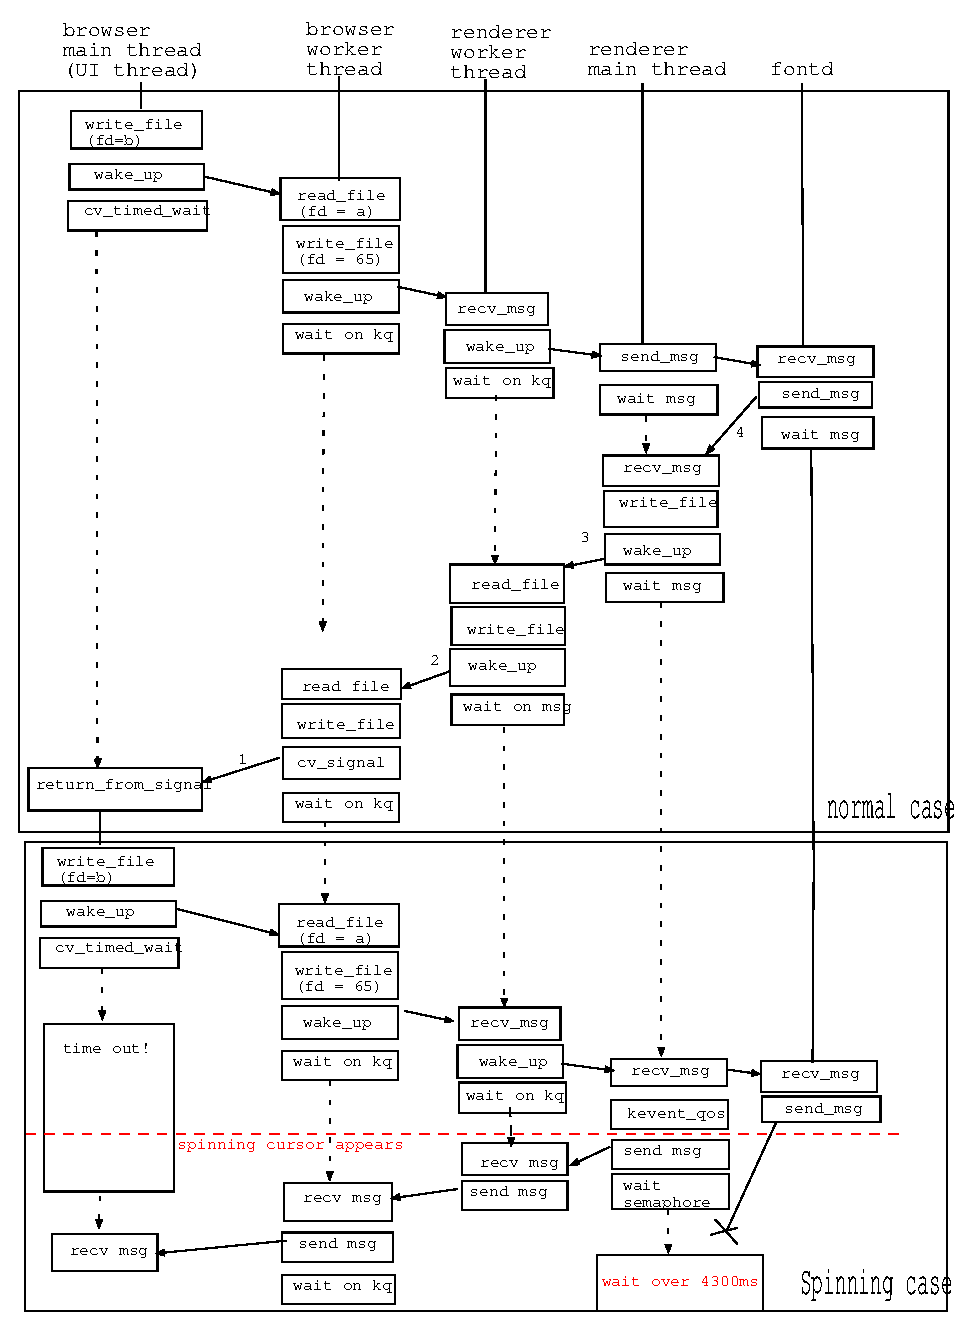
\includegraphics[width=1.0\linewidth]{chromium_case_study.eps}
    \caption{Chromium case study.}
    \label{fig:chromium-trace}
\end{figure}



The chromium bug has been reported multiple times in the chromium bug report.
It was initially a deadlock bug in which the main thread in the browser is waiting on a condition variable.
As no one knows how the deadlock triggered, timeout is added as a programming trick to eliminate the deadlock.
However, the bug is not resolved, and the main thread would always timeout in some situation for a relatively long time.
Hence, a further patch introduced cache mechanism to alleviate the non-responsive, which did not solve the problem from the root cause and the main thread still get hang from time to time.

The bug of the System Preferences is exposed by an app called DisableMonitor.
The app can change some system settings and eventually reveal the inappropriate displayer management in CoreGraphics Framework.

The spinning wait cursor is a painful sight for Mac users, signifying that the application is non-responsive.
It usually remains for munites, leaving the users at a loss .                    

Argus shreds light on the design of the spinning wait cursor with the backward path slicing.
We begin the path from the node where the spindump, a hang reporting tool, is launched,  
considering the spindump shares the same triggering condition.
As is shown in Figure \ref{fig:spincursor}, the spindump is launched by the message from WindowServer, after the WindowServe received message from the NSEvent thread of targeted Application.

We further added call stacks for the messages and revealed two shared variables are critical in the desgin, "is\_mainthread\_spinning" and "dispatch\_to\_mainthread".
The NSEvent thread of the targeted App fetches CoreGraphics events from WindowServer, converts and creates NSEvents for the main thread.
If the mainthread is not spinning by checking "is\_mainthread\_spinning", "dispath\_to\_mainthread" is set and a timer is armed.
If the main thread processes the next event before the timer fires, nothing happens and the timer gets reset.
Otherwise, NSEvent thread sends a message to WindowServer from the timer,
and WindowServer notifies the CoreGraphics to draw spinning cursor over the application window.

\subsection{Chromium IME responsive}
One of the long lasting performance issue in chromium is hanging caused by the non-English input.
When users try to type non English to textFields, such as search box,
the main thread of the browser becomes non responsive.
With lldb it is not hard to tell that the main thread get stuck on FindFirstRect,
where the main thread waits for the signal of condition variable.
According to the history in bug report, the developers realized there were deadlocks somewhere.
However, it was hard to pinpoint due to the multiprocess and multithread programing paradigms.
As a result, timeout was added to prevent the deadlock, but not the long latency.
Although a further bug patch introducing cache helps to eliminate the long hanging mostly, 
the performance issue still appears from time to time.
The senario we can reproduce is to open the website of yahoo and quickly type Simplified Chinese.

The ground true we reveal with out tool is as shown in the picture XXX.
In chromium, there are one browser process and multiple renderer processes.
The main thread of the browser process try to get the caret position.
It sends out the message and wait for the reply on a condition variable.
Usually, a worker thread in the browser process will return the firstrect and wake up the main thread.
Howeve, it requires the message from the main thread of a renderer process to proceed.
Without the message from the renderer process, the worker thread is not able to signal the main thread,
thus, the main thread in will always time out.

Our trace tool will collect the data system wide, therefore, all the thread relationships are captured.
With the trace log size, both the hanging case and non-hanging case are recorded.
From the shared condition variable between threads, we are able to align the logs of the two cases,
and discover the missing message in the hanging case.

As we known the unresponsive of the main thread in the renderer process,
we further consult the analyzed trace log and observe that it is waiting on a semaphre,
and eventually waken by the main thread of the browser process.

Our tool further reveal the root cause of the livelock with conditional debugging.
We can either binary instrument or modify the source code to make the renderer thread accept the attachment of lldb.
The concrete call stacks from lldb disclose the task processing in the renderer thread is related to running javascript.

\subsection{System Preferences spin}
System Preferences is the application in MacOS for users to modify various settings.
Displays in the Panel allows user to rearrange the position of displays, but it does not support the disabling of a montor online.
DisableMonitor is an application used to complete the function, easily disabling/enabling  monitors withou unplug them.
Surprisingly, the operation of DisableMonitor exposed a performance bug in System Preferences.
If we disable an external monitor and arrange them afterward, the window System Preferences freezes for seconds.
We enabled Argus on the background and collect the data by normally arranging the displays and reapeating the spinning sequence.

It is not hard to tell the spinning node in the UI thread with our tool.
However, to find the normal node corresponding to the spinning node is not straightforward as in the previous case.
The execution segment includes two types of events: ``\v{mach\_msg}'' and ``\v{thread\_switch}''.
Both of them are used to waiting for the data available ping.
The semantics of the execution segment is not descriptive enough
to identify the normal nodes in the same operation stage.

In the case we detected the intensive timeout in the node,
our search algorithm identify the corresponding normal node by searching the similarity of their proceding nodes.
We find out the path of the normal path as shown in the Figure \ref{fig:path slicing for system preference}.
Our lightweight callstacks were used to verify the correctness of the findings.

The normal node showed it proceeded to \textit{displayReconfigured} after received the message with id 29675.
The spinning node fell into the ``\v{thread\_switch}'' after receiving the message with the same id,
and end up to send message for the available datagram ping with \textit{CGSSnarfAndDispatchDatagrams} again.
The proceding nodes before them sent message to WindowServer for \textit{activeDisplayNotificationHandler}.

With the result, we initiate the concrete debugging by filling the debugging script with the APIs reported.
We set the method \textit{activeDisplayNotificationHandler} as a beakpoint where the script begins debugging.
\textit{displayReconfigured} and \textit{CGSSnarfAndDispatchDatagrams} are recorded to indicate the end of debugging for the normal case and spinning case respectively.

Our debugging scripts ran within the confined range for both the noraml and the spinning execution.
The logs are generated as shown in Figure \ref{fig:step debug log for system preferences}.
By diff the two logs, it is easy for the user to notice the differen braches in \textit{display\_notify\_proc},
which is resulted from its prameter standing for the datagram type.

We make use of the diassembly tool, and reveals the story in the background.
Datagrams from the WindowServer makes applications to handle notifications.
The datagram causes difference are used to finish display reconfiguration for System Preference.
However, in the spinning case the reconfiguration got initiated but not completed.
The main thread leveraged thread\_switch to wait for the flollowing datagram and resulted in a freeze.
As a conclusion, the handler display\_notify\_proc is not appropriately implemented.

